% 第三章 结果（每一章必须另页起）
\chapter{结果}
正文文字正文文字正文文字正文文字正文文字正文文字正文文字正文文字正文文字正文文字正文文字正文文字正文文字正文文字正文文字正文文字正文文字正文文字正文文字正文文字正文文字正文文字正文文字正文文字。

\section{标题}
正文文字正文文字正文文字正文文字正文文字正文文字正文文字正文文字正文文字正文文字正文文字正文文字正文文字正文文字正文文字正文文字正文文字正文文字正文文字正文文字正文文字正文文字正文文字正文文字。

\subsection{标题}
正文文字正文文字正文文字正文文字正文文字正文文字正文文字正文文字正文文字文字。

\begin{figure}[htbp]
    \centering
    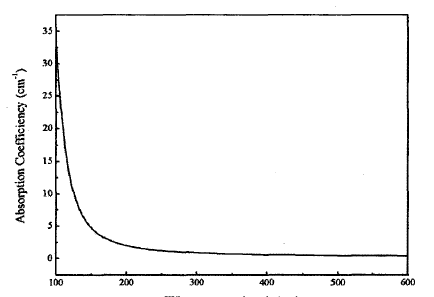
\includegraphics[width=0.62\textwidth]{image/image1.png}
    \bicaption{单图示例}{Single image example}
    \label{fig:single-image-example}
    \fignote{注：如有需要可对图片进行注释说明，标尺内容，英文简称，统计值等，不用可省略。\par 图片来源：如需对图片来源进行说明，请参照此格式，不用可省略。}
\end{figure}

正文文字正文文字正文文字正文文字正文文字正文文字正文文字正文文字正文文字正文文字正文文字正文文字正文文字正文文字正文文字正文文字正文文字正文文字正文文字正文文字正文。

% 如果一个图由两个或两个以上分图组成时，各分图分别以(a)、(b)、(c)……作为图序，
% 并须有分图名，分图名直接列在各自分图的正下方，主图名列在所有分图的下方正中。

\section{标题}
正文文字正文文字正文文字正文文字正文文字正文文字正文文字正文文字正文文字正文文字正文文字正文文字正文文字正文文字正文文字正文文字正文文字正文文字正文文字正文文字正文。

\subsection{标题}
正文文字正文文字正文文字正文文字正文文字正文文字正文文字正文文字正文文字正文

\subsubsection{标题}
\begin{figure}[htbp]
    \centering
    \begin{minipage}[t]{0.48\textwidth}
        \centering
        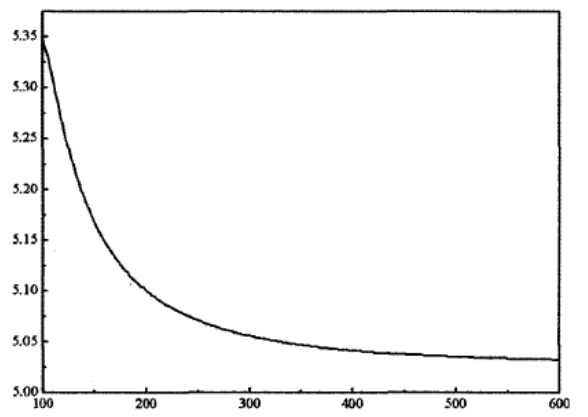
\includegraphics[width=\textwidth]{image/image2(a).png}
        
        {\songti\rmfamily\xiaosi (a)\quad 分图示例一\par}
    \end{minipage}\hfill
    \begin{minipage}[t]{0.48\textwidth}
        \centering
        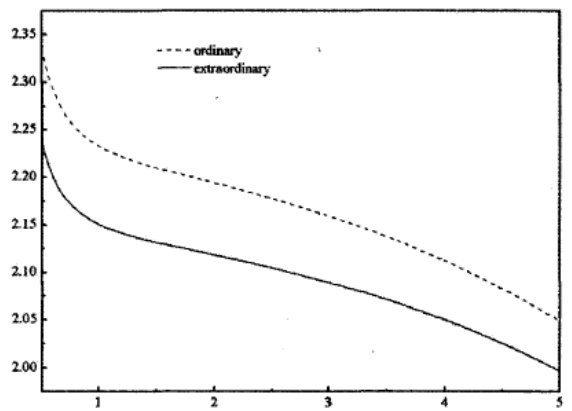
\includegraphics[width=\textwidth]{image/image2(b).png}
        
        {\songti\rmfamily\xiaosi (b)\quad 分图示例二\par}
    \end{minipage}
    \bicaption{双图示例}{Two-image example}
    \label{fig:two-image-example}
\end{figure}

\section{标题}
正文文字正文文字正文文字正文文字正文文字正文文字正文文字正文文字正文文字正文文字正文文字正文文字正文文字正文文字正文文字正文文字正文文字正文文字正文文字正文文字正文。
